\documentclass[a4paper, 12pt]{article}

\usepackage{wrapfig}
\usepackage{graphicx}
\usepackage{mathtext}
\usepackage{amsmath}
\usepackage{siunitx} % Required for alignment
\usepackage{multirow}
\usepackage{rotating}
\usepackage{float}
\usepackage{booktabs}
\usepackage{color, colortbl}

\usepackage[russian]{babel}

%Light gray:
\definecolor{Gray}{gray}{0.9}

\graphicspath{{pictures/}}

\title{\begin{center}Лабораторная работа №1.1.1\end{center}
Определение удельного сопротивления нихромовой проволки}
\author{Гёлецян А.Г.}
\date{\today}

\begin{document}
    \pagenumbering{gobble}
    \maketitle
    \newpage
    \pagenumbering{arabic}

    \section{Введение}
    \textbf{Цель работы:}
    \begin{itemize}
        \item измерить удельное сопротивление нихромовой проволки
        \item вычислить систематические и случайные ошибки
    \end{itemize}

    \vspace{1cm}

    \textbf{В работе используются: }
    \begin{itemize}
        \item линейка
        \item штангенциркуль
        \item микрометр
        \item отрезок проволки из нихрома
        \item амперметр
        \item вольтметр
        \item мост постоянного тока
    \end{itemize}

    \newpage
    \section{Ход работы}
    \paragraph{}
    Для расчета удельного сопротивления измерим сопротивление проволки с известной геометрией и высчитаем удельное сопротивление по формуле
    \begin{equation}
        \rho = \frac{R}{l}\frac{\pi d^{2}}{4}\
    \end{equation}
    где $R$ - сопротивление проволки, $l$ -длина проволки, $d$ - диаметр проволки.

    \paragraph{}
    Измерения мы буедм проводить для 3х длин проволки - $50, 30, 20$ $см$.
    \paragraph{}
    Для начала измерим толщину проволки, учитывая что из за неровностей она меняется по длине проволки, поэтому измерим его в нескольких точках и усредним.
    При измерении штангенциркулем везде получаем одно и то же значение

    \[d_{шц} = (0.35 \pm 0.025) мм\]

    \vspace{0.5cm}

    \begin{center}
        При измерении микрометром получаем значения
    \end{center}

    \begin{table}[H]
        \begin{center}

         \begin{tabular}{|c|c|c|c|c|c|c|c|c|c|}
            \hline
            \multirow{2}{*}{\textbf{$d, мм$}}
            & 0.35 & 0.35 & 0.35 & 0.35 & 0.35 & 0.34 & 0.35 & 0.36 & 0.35\\
            \cline{2-10}
            & 0.36 & 0.35 & 0.36 & 0.35 & 0.34 & 0.36 & 0.35 & 0.36 & - \\
            \hline
        \end{tabular}
            \caption{Измерения диаметра проволки микрометром}
        \end{center}

    \end{table}
    \paragraph{}
    Усреднив значения из таблицы, посчитав дисперсию выборки и суммировав её с систематической ошибкой $\Delta d_{сист} = 0.005мм$ получаем

    \[d_{мр} = (0.352 \pm 0.005)мм\]

    \paragraph{}
    Сразу же подсчитаем площадь поперечного сечения для обоих случаев

    \begin{align*}
        S_{шц} &= (0.096 \pm 0.01) мм^2 \\
        S_{мр} &= (0.097 \pm 0.003)мм^2
    \end{align*}

    \newpage

    \begin{table}[H]
        \begin{center}

        \begin{tabular}{|l|r|r|r|r|r|r|}
        \hline
        $l, см$ & \multicolumn{2}{c|}{20} & \multicolumn{2}{c|}{30} & \multicolumn{2}{c|}{50} \\
        \hline
        {№} &      $U, мВ$ &        $I, мА$&      $U, мВ$ &         $I, мА$ &    $U, мВ$ &         $I, мА$ \\
        \hline \rowcolor{Gray}
        1  &   44 &   21.043 &   72 &   22.94 &   64 &   12.25 \\
        2  &  108 &   52.54  &  124 &   39.32 &  124 &   23.49 \\\rowcolor{Gray}
        3  &  152 &   72.92  &  150 &   47.11 &  180 &   34.08 \\
        4  &  208 &   99.78  &  200 &   63.61 &  216 &   40.65 \\\rowcolor{Gray}
        5  &  288 &  136.66  &  260 &   81.57 &  272 &   51.03 \\
        6  &  352 &  167.88  &  296 &   93.15 &  328 &   61.63 \\\rowcolor{Gray}
        7  &  400 &  190.63  &  328 &  103.25 &  360 &   68.02 \\
        8  &  448 &  213.55  &  392 &  122.90 &  388 &   72.11 \\\rowcolor{Gray}
        9  &  536 &  255.11  &  456 &  142.73 &  452 &   85.10 \\
        10 &  580 &  277.14  &  500 &  157.06 &  484 &   90.78 \\\rowcolor{Gray}
        11 &      &          &  556 &  174.32 &  536 &  100.23 \\
        12 &      &          &      &         &  588 &  110.10 \\
        \hline
        \end{tabular}
            \caption{Измерении зависимости $U(I)$ при различных $l$}
        \end{center}

    \end{table}

    \paragraph{}

    \begin{wrapfigure}{l}{0.5\linewidth}
        \begin{center}
            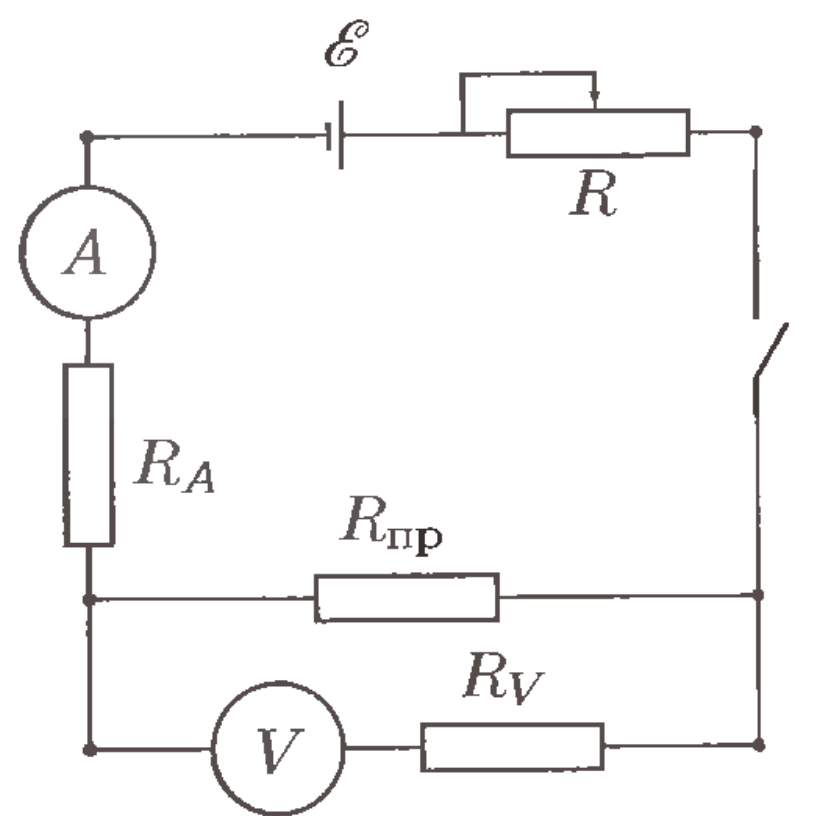
\includegraphics[scale=0.3]{sxema.png}
            \caption{Схема установки}
        \end{center}
    \end{wrapfigure}
    Измерения будем проводить по схеме ниже. Обозначим показания вольтметра как $U$, а амперметра как $I$. Легко получить формулу для $R_{пр}$
    \[R_{пр} = \frac{U}{I}\left(1 + \frac{U/I}{R_{v}}\right)\]
    \paragraph{}
    Из чарактеристик вольтметра знаем что сопротивление вольтметра порядка $k\Omega$, поэтому поправка $\frac{U/I}{R_v}$ порядка $0.5\%$, что больше относительных погрешностей вольтметра и амперметра в $2.5$ раза. Исходя из этого пренебрежем влиянием сопротивления вольтметра и воспользуемся приближенной формулой
    \[R_{пр}\approx\frac{U}{I}\]
    \newpage
    \paragraph{}
    Для нахождения сопротивления построим график $U(I)$, и из наклона прямой найдем сопротивление. Из графика получаем следующие данные.


    \begin{table}[H]
        \begin{center}

        \begin{tabular}{|l|r|r|r|}
        \hline
        $l, см$          &  20 & 30 & 50 \\
        \hline
        $R_{пр}, \Omega$ &  $2.102\pm0.008$ & $3.199\pm0.011$  & $5.357\pm0.031$\\
        \hline
        \end{tabular}
            \caption{Расчетные $R_{пр}$ от $l$}
        \end{center}

    \end{table}

    \paragraph{}
    Сравним с данными измерении от моста Р4833.

    \begin{table}[H]
        \begin{center}

        \begin{tabular}{|l|r|r|r|}
        \hline
        $l, см$          &  20 & 30 & 50 \\
        \hline
        $R_{пр}, \Omega$ &  2.2949 & 3.3843 & 5.4173 \\
        \hline
        \end{tabular}
            \caption{$R_{пр}$ от $l$ по измерениям Р4833}
        \end{center}

    \end{table}

    \paragraph{}
    Рассмотрим на сколько процентов расчетные сопротивления меньше имерянных.

    \begin{table}[H]
        \begin{center}

        \begin{tabular}{|l|r|r|r|}
        \hline
        $l, см$          &  20 & 30 & 50 \\
        \hline
        $\varepsilon, \%$ &  8.4 & 5.5 & 1.1 \\
        \hline
        \end{tabular}
            \caption{Различие между сопротивлениями}
        \end{center}

    \end{table}

    \paragraph{}
    Эти различия очень большие и никак не объясняются погрешностями. Так как график идеально линейный, то на вряд ли это из за плохих измерении. Тут есть 2 объяснения. Первое это то что мост выдает сопротивление, которое отличается от реального умножением на константу, второе это то же самое но только с вольтметром. Я больше ссылаюсь на второй вариант, поэтому для расчета удельного сопротивления я буду брать сопротивления с моста.
    \paragraph{}
    Погрешность моста в диопазоне измерении $\pm0.01\Omega$ (рассчитано по классу точности).
    Воспользуемся следующими формулами для подсчета удельного сопротивления и его погрешности.
    \begin{align*}
        \rho &= \frac{RS}{l}\\
        \Delta\rho &= \rho\sqrt{\left(\frac{\Delta R}{R}\right)^2 + \left(\frac{\Delta S}{S}\right)^2 + \left(\frac{\Delta l}{l}\right)^2}
    \end{align*}
    \paragraph{}
    Для площади сечения $S$ воспользуемся значением, полученным с помощью микрометра. Подставляя числа получаем


    \begin{table}[H]
        \begin{center}

        \begin{tabular}{|l|r|r|r|}
        \hline
        $l, см$          &  20 & 30 & 50 \\
        \hline
        $\rho, 10^{-4}\Omegaсм$ &  1.11 & 1.09 & 1.05 \\
        \hline
        $\Delta\rho, 10^{-4}\Omegaсм$ &  0.04 & 0.03 & 0.03 \\
        \hline
        \end{tabular}
            \caption{Различие между сопротивлениями}
        \end{center}

    \end{table}

    Как ответ запишем среднее  \[\rho = (1.08 + 0.04)10^{-4}\Omegaсм, \varepsilon_{\rho} \approx 4\%\]

    \section{Заключение}
    Значение удельного сопротивления совпадает с табличными значениями для нихрома. Значении сопротивлении измерянных косвенным методои оказались в среднем на $5\%$ ниже реальных, что скорее всего объясненяется либо некалиброванностью вольтметра, либо его аномальной малостью внутреннего сопротивления вольтметра (порядка $100\Omega$). В любом случае даже использовав заниженные сопротивления приходим к тому же выводу что проволка действительно нихромовая.
    \newpage


    \begin{table}
        \begin{center}

        \begin{tabular}{|l|c|}
        \hline
        Устройство & Вольтметр аналоговый, магнитлэлектрический \\\rowcolor{Gray}
        \hline
        Класс точности &  0.2\\
        \hline
        Предел измерении&  600мВ \\\rowcolor{Gray}
        \hline
        Цена деления&  4мВ/дел \\
        \hline
        Чувтствительность &  250дел/В \\\rowcolor{Gray}
        \hline
        Абсолютная погрешность&  2мВ \\
        \hline
        Внутреннее сопротивление&  $~2000\Omega$\\
        \hline

        \multicolumn{2}{c}{} \\\rowcolor{Gray}


        \hline
        Устройство & Амперметр цифровой\\
        \hline
        Класс точности &  0.2\\\rowcolor{Gray}
        \hline
        Предел измерении&  2А \\
        \hline
        Абсолютная погрешность&  Единица младшего разряда \\\rowcolor{Gray}
        \hline
        Внутреннее сопротивление&  $1.2\Omega$\\
        \hline
        \end{tabular}
            \caption{Характеристики измерительных приборов}
        \end{center}

    \end{table}

    \newpage
    \begin{sidewaysfigure}
        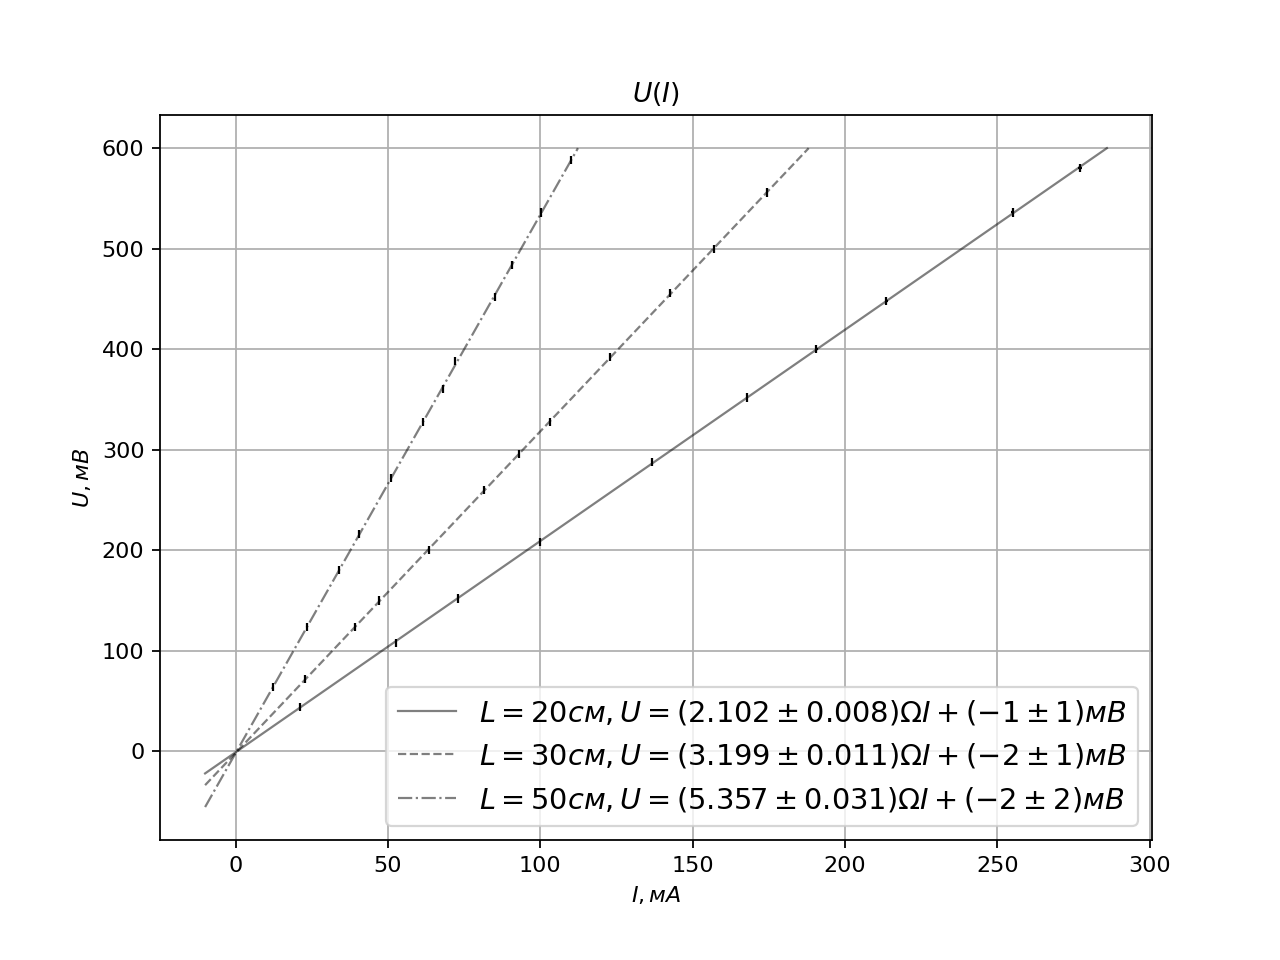
\includegraphics[scale=1]{grafik.png}
        \caption{График зависимости $U(I)$}
    \end{sidewaysfigure}
\end{document}
